\documentclass{article}
\usepackage[UTF8]{ctex}
\usepackage{extarrows}
\usepackage{amsmath,amssymb,amsthm,mathtools}
\usepackage [dvipsnames]{xcolor}
\usepackage{graphicx}

\begin{document}
\title{Abaqus 6.14-1 Ubuntu install tutorial}
\author{hu tianyun}
\maketitle
经过许多许多次的尝试和错误,终于找到了能够在 Linux 下安装 ABAQUS 的文件和破解之法。
\section{Document \textit{VS} Product install} % (fold)
\label{sec:document_vs_product_install}
	Document 的安装与 ABAQUS 产品的安装没有联系,安装时注意是安装的是哪一个。
	能安装 Product 的文件夹:

	\begin{figure}[!htbp]
	\centering
 		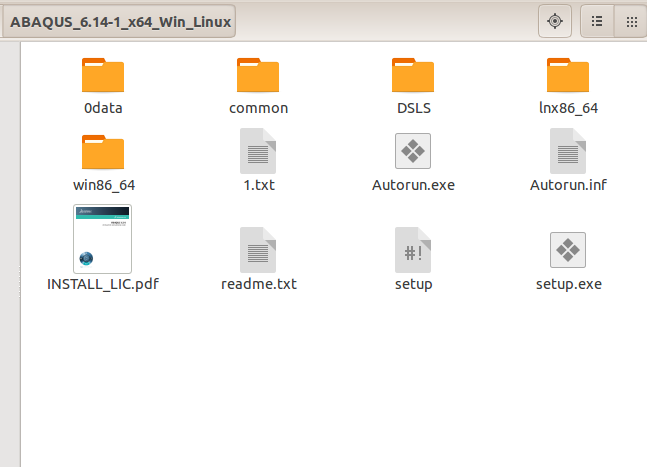
\includegraphics[width = .8\textwidth]{abaqus_install_ubuntu.png}
		\caption{abaqus  File}
		\label{abaqus_install_ubuntu}
	\end{figure}

	
\section{ABAQUS 产品安装步骤:} % (fold)
\label{sec:abaqus_installstep_}

	\begin{enumerate}
	\item License 的破解,复制 simulia 文件夹 到 /opt 或者 /usr 目录 下, 注意 ABAQUS.lic 中 的 hostname 改成 本机的名字 例如 admin-pc 或 xxx-pc , 其他的不动如 \textbf{270011} 等数字不改变它们。
	\item 先用  sudo chmod -R 777 file\_name/ 将文件夹下的文件改成可执行文件,使用 lmgrd -c ABAQUS.lic 启动 License。
	\item ./setup 启动安装,详情可参考自带安装步骤,在License name 中填入在 ABAQUS.lic 中修改的hostname 和  \textbf{没有动过的port-num} 如  270011@ xxx-pc,一路next 直到安装完毕。
	\item 破解时如果遇到 license 无法启动或者 报错,端口被占用等情况时,可使用 
	killall -9 ABAQUSLM 清除,或使用  lmstat , lmreread , lmdown 来清除端口。
	在此次安装中虽然也遇到了不能启动破解的情况,但是因为 license name 填写正确,仍然强行安装成功了。	
	\end{enumerate}

	Some problems:\\
	有时会遇到一些包没有安装,Google 下安装就行。

	例如: sudo apt-get install libjpeg62

\section{ABAQUS 的启动} % (fold)
\label{sec:abaqus_start}
	在进入安装完成的文件夹中的 Commend , 启动命令\\
	 sudo XLIB\_SKIP\_ARGB\_VISUALS=1 'install-file/Commands/abaqus' cae

	 或者在 sudo ~/.bashrc 中写入\\
	 alias abaqus='sudo XLIB\_SKIP\_ARGB\_VISUALS=1 'install-file/Commands/abaqus' cae'
% section abaqus_的启动 (end)

\end{document}

